\section{Theorie}
\label{sec:Theorie}
\subsection{Ziel}
Mit gepulster Kernspinresonanz (NMR) kann der zeitliche Verlauf der Magnetisierung
einer Probe, unter Einwirkung eines Hochfrequenzfeldes untersucht werden. Die
dabei auftretenden Relaxationsprozesse werden unter Verwendung zweier
charakteristischer Relaxationszeiten beschrieben.
Aus diesen Größen wird die Diffusionskonstante von Wasser bestimmt.
\subsection{Magnetisierung einer Probe}
Durch ein Magnetfeld $\vec{B_0}=B_0 \vec{e_\text{z}}$, hier in Richtung der z-Achse,
spalten die Energieniveaus
in $2I+1$ äquidistante Unterniveaus auf. Dabei beschreibt $I$ die Spinquantenzahl.
Mit der Orientierungsquantenzahl $m$ mit $-I \leq m \leq I$ kann zwischen
den Zuständen unterschieden werden. Wenn sich die Probe im thermischen
Gleichgewicht mit der Umgebung befindet, sind die Niveaus gemäß der Boltzmannverteilung
unterschiedlich besetzt. Es ergibt sich eine mittlere Kernspinpolarisation, die
für Protonen mit $I=1/2$  und unter der Annahme $m \gamma B_0 \hbar \ll k_\text{B} T$ mit
\begin{equation}
  \langle I_{\text{Z}} \rangle= -\frac{\hbar^2}{4}\frac{\gamma B_0}{k_\text{B} T}
\end{equation}
genähert werden kann. Hier bezeichnet $\gamma$ das gyromagnetische Verhältnis des Kerns,
$k_\text{B}$ die Boltzmann-Konstante, $T$ die Temperatur
und $\hbar$ das Plancksche Wirkungsquantum.
Durch die Kernspinpolarisation wird über die magnetischen Momente $\vec{\mu_\text{I}}$ eine Magnetisierung
der Probe erzeugt. Der Betrag der Magnetisierung in Richtung des Magnetfelds ist
\begin{equation}
  M_0 = \frac{1}{4} \mu_0 \gamma^2 \frac{\hbar^2}{k_\text{B}} N \frac{B_0}{T},
\end{equation}
wobei $\mu_0$ die Permeabilität des Vakuums und
$N$ die Anzahl der Momente pro Volumeneinheit bezeichnet.\\
Um das zeitliche Verhalten der Probenmagnetisierung zu untersuchen, kann klassisch
vorgegangen werden, da die Anzahl an Einzelmomenten $N$ mit etwa $10^{28}/$m$^3$
groß genug ist.
Auf die Probenmagnetisierung $\vec{M}$ wirkt im externen Magnetfeld $\vec{B_0}$ ein Drehmoment
$\vec{D}= \vec{M}\times \vec{B_0}$.  Dies führt zu einer Präzessionsbewegung um
die Richtung des Magnetfelds. Die Frequenz dieser Präzessionsbewegung wird
Larmor-Frequenz genannt und mit
\begin{equation}
  \omega_{\text{L}}= \gamma B_0 .
\end{equation}
Wird die Probenmagnetisierung durch ein Äußeres Feld aus ihrer Gleichgewichtslage entfernt, relaxiert sie nach
Ende der Störung wieder in die Ausgangslage zurück. Die Relaxion
wird über die Blochschen-Gleichungen
\begin{equation}
  \begin{split}
    \frac{\symup{d} M_\text{z}}{\symup{d} t} &= \frac{M_0 - M_\text{z}}{T_1} \\
    \frac{\symup{d} M_\text{x}}{\symup{d} t} &=
      \gamma B_0 M_\text{y} - \frac{M_\text{x}}{T_2} \\
    \frac{\symup{d} M_\text{y}}{\symup{d} t} &=
      - \gamma B_0 M_\text{x} - \frac{M_\text{y}}{T_2},
  \end{split}
  \label{eq:Bloch-Gleichungen}
\end{equation}
beschrieben.
Die auftretenden charakteristischen Zeitkonstanten $T_1$ und $T_2$ beschreiben dabei unterschiedliche
Effekte.  Die  sogenannte longitudinale oder
Spin-Gitter-Relaxationszeit $T_1$ bezeichnet die Veränderung des Magnetfelds parallel
zur Achse des Magnetfeldes. Sie beschreibt auch die Zeit in der bei Festkörpern Energie aus dem Kernspinsystem
in Gitterschwingungen umgewandelt wird. Die Bezeichnung wird auch bei flüssigen Proben beibehalten.
Die Zeitkonstante $T_2$ wird transversale oder Spin-Spin-Relaxationszeit bezeichnet. Diese Größe
beschreibt die Änderung der senkrechten Komponente der Probenmagnetisierung zur
Richtung des externen magnetischen Feldes. Durch Wechselwirkungen der Spins mit ihren
Nachbarn nimmt die Magnetisierung senkrecht zu $\vec{B}$ ab. \\
Um die Probenmagnetisierung aus dem Gleichgewicht zu entfernen wird
ein Hochfrequenzfeld $\vec{B_{\text{HF}}}$ senkrecht zu $\vec{B_0}$ angelegt. Dieses kann
in zwei zirkular polarisierte Felder mit den Frequenzen $\pm \omega$ zerlegt werden. Liegt die positive
Frequenz in der Nähe der Larmorfrequenz, so kann der Einfluss des anderen Feldes vernachlässigbar.
Das Hochfrequenzfeld lässt sich somit durch
\begin{equation*}
  B_\text{x} = B_1 \cos\!\left(\omega t\right) \quad\quad
  B_\text{y} = B_1 \sin\!\left(\omega t\right)
\end{equation*}
darstellen.
Um die Blochschen Differentialgleichungen \ref{eq:Bloch-Gleichungen} zu Lösen, wird das System in ein
Koordinatensystem transformiert, das mit der Frequenz $\omega$ um $\vec{B}_0$
rotiert. Im neuen System $\left\{x', y', z'\right\}$
ist $\vec{B}_\text{HF}$ zwar konstant (hier in $x'$-Richtung),
jedoch sind die Einheitsvektoren zeitabhängig.
Durch das Einführen eines effektiven Magnetfeldes
\begin{equation}
  \vec{B}_\text{eff} = \vec{B}_0 + \vec{B}_1 + \frac{\vec{\omega}}{\gamma}
\end{equation}
lässt sich die zeitliche Änderung der Probenmagnetisierung durch
\begin{equation}
  \frac{\symup{d} \vec{M}}{\symup{d} t} =
  \gamma \left(\vec{M} \times \vec{B}_\text{eff}\right)
\end{equation}
darstellen, was eine Präzession von $\vec{M}$ um die Feldrichtung $\vec{B_{\text{eff}}}$ beschreibt.
Im Resonanzfall ist die Frequenz des Hochfrequenzfeldes die Larmorfrequenz und die Magnetisierung
präzediert mit einem Öffnungswinkel von 90° um die $\vec{B_1}$-Achse.
Wird das Hochfrequenzfeld für die Zeit
\begin{equation}
  \Delta t_{90} = \frac{\pi}{2 \gamma B_1}
  \quad\quad (\text{mit } \Delta t_{90} \ll T_1, T_2)
  \label{eq:t90}
\end{equation}
eingeschaltet, dreht sich die Magnetisierung aus der $z$-Richtung in die
$y$-Richtung.
Ebenso lässt sich ein 180°-Puls realisieren, der die Magnetisierung
in die negative $z$-Richtung dreht.
\subsection{Methoden zur Messung der Relaxationszeiten}
\paragraph{Der freie Induktionsfall}
Wird die Probenmagnetisierung um 90° aus der Gleichgewichtslage entfernt, präzediert
sie in der Ebene senkrecht dazu. Durch die Relaxationsprozesse kehrt die Magnetisierung
in die Ausgangslage. Dies wird freier Induktionsfall genannt und liegt an
dem statischen Magnetfeld $\vec{B_0}$. Dies hat nicht für alle Spins in einer realen Probe
den selben Betrag. Dies kann einerseits durch den Einfluss der Dipolfelder der benachbarten Spins kommen,
oder daran liegen, das ein reales Feld zwangsläufig inhomogen ist. Daraus resultiert eine
Verteilung von Larmorfrequenzen für die einzelnen Spins, was zu einer Dephasierung der
Spins untereinander und infolge dessen
zu einem Zerfall der transversalen Magnetisierung führt. Aus diesem Grund kommt zu der
transversale Zeitkonstante $T_2$ noch eine weitere Zeitkonstante $T_{\Delta B}$ hinzu, die
aus der apparativen Inhomogenität des Magnetfelds entsteht. Dies macht den
freien Induktionsfall häufig kompliziert zu beschreiben, und die Berechnung von $T_2$ ist nur
für $T_{\Delta B} \ll T_2$ möglich.
\paragraph{Das Spin-Echo-Verfahren}
Der Störeffekt der Inhomogenität des Magnetfelds kann durch das Spin-Echo-Verfahren
korrigiert werden, wenn die Inhomogenität zeitlich konstant ist. Hierzu sind zwei Hochfrequenzpulse
notwendig. Wenn das Magnetfeld $\vec{B_0}$ in z-Richtung zeigt, dann dreht ein
erster 90° Puls die Magnetisierung in die y-Richtung.
\begin{figure}[H]
  \centering
  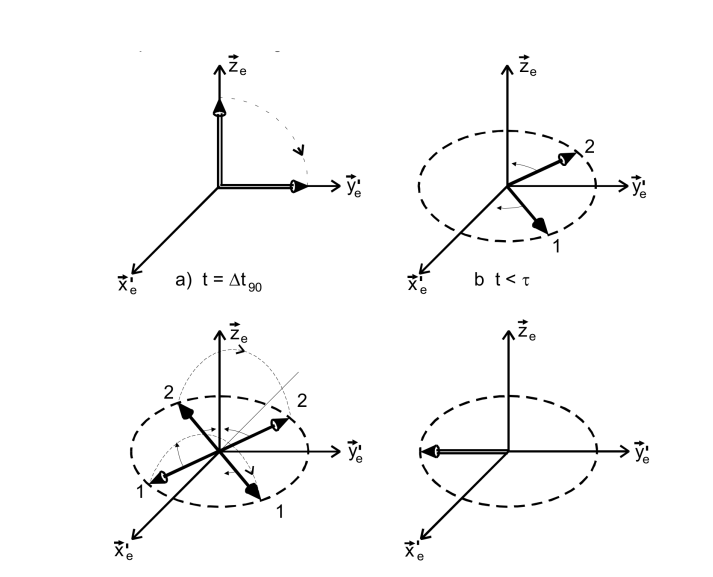
\includegraphics[width=0.8\textwidth]{pics/SEM.png}
  \caption{Darstellung des Verhalten der Spins bei dem Spin-Echo-Verfahren \cite{Anleitung}.}
  \label{fig:SEM}
\end{figure}
Dort tritt während der
Präszession, im Zeitraum $ \tau \ll \Delta t_{90}$ um die z-Achse, eine Dephasierung auf.
Nach einer zeit $T_{\Delta B}$ ist praktisch kein Induktionssignal mehr zu messen, da
die Spins zu weit auseinander gelaufen sind. Am Ende des Zeitraums $\tau$ wird
ein 180°-Puls auf die Probe gegeben. Dadurch werden die Spins um die x-Achse gedreht und
laufen deswegen wieder zusammen. Nach einem weiteren Zeitraum $\tau$ sind die
Spins wieder in Phase. Der zeitliche Verlauf ist in Abbildung \ref{fig:SEM} dargestellt.
Da das transversale Magnetfeld mit der Relaxationszeit $T_2$ abklingt, erfolgt auch ein
Abfall in der Signalstärke. In Abbildung \ref{fig:Signal} ist der zeitliche Verlauf der
Signalstärke dargestellt. Da auch irreversible Dephasierungsprozesse auftreten, wird
Signal nach $2\tau$ nicht mehr so hoch sein wie am Anfang. Die
Höhe des Spin-Echos$M_{\text{Y}}$ in Abhängigkeit der Zeit wird durch eine
Exponentialfunktion
\begin{equation}
  M_{\text{Y}}=M_0 \exp{(-t/T_2)}
\label{eq:MYT2}
\end{equation}
beschreiben.
\begin{figure}[H]
  \centering
  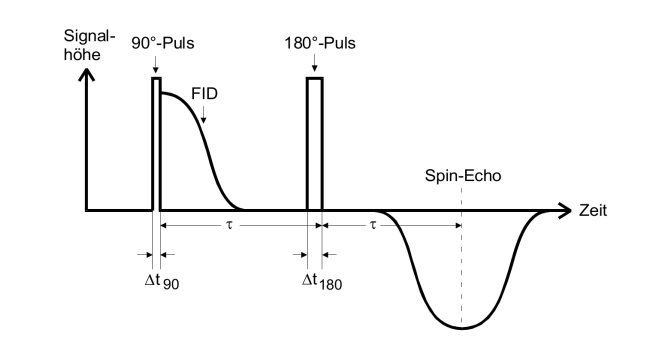
\includegraphics[width=0.6\textwidth]{pics/Signalverlauf.png}
  \caption{Darstellung Signalverlaufs bei dem Spin-Echo-Verfahren \cite{Anleitung}.}
  \label{fig:Signal}
\end{figure}
\paragraph{Die Carr-Purcell- und die Meiboom-Gill-Methode}
Um nicht nach jeder Messung des Spin-Echos warten zu müssen, bis die Magnetisierung wieder
in der Gleichgewichtslage ist, nutzt die Carr-Purcell Methode eine Reihe von
180°-Pulsen im äquidistanten Abstand von $2\tau$. Der Signalverlauf ist in Abbildung
\ref{fig:CPM} dargestellt.
\begin{figure}[H]
  \centering
  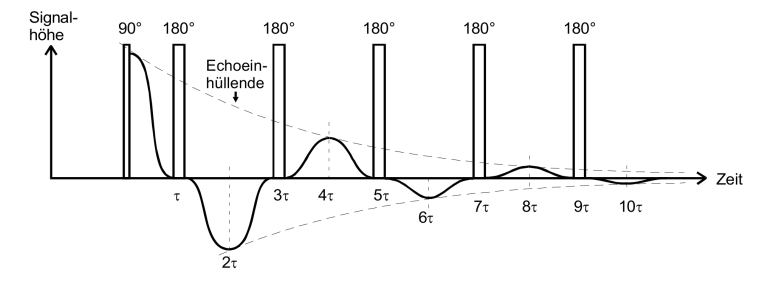
\includegraphics[width=0.8\textwidth]{pics/CPM.png}
  \caption{Darstellung des Signalverlaufs bei der Carr-Purcell-Methode \cite{Anleitung}.}
  \label{fig:CPM}
\end{figure}
Die Spins werden immer zum Zeitpunkt $2n\tau$ wieder fokussiert,
jedoch nimmt die Amplitude exponentiell ab. Daraus lässt sich $T_2$ bestimmen, wenn
die Justage der 180°-Pulse exakt ist. Ist dies nicht der Fall, addieren sich die
Fehler bei jedem Schritt, wodurch ein geringerer Wert als $T_2$ gemessen wird.\\
Bei der Meiboom-Gill-Methode wird dieses Problem behoben, in dem zusätzlich zu den 180°-Pulsen
noch phasenverschobene 90°-Pulse genutzt werden. In Abbildung \ref{fig:Meiboom}
ist das Verfahren dargestellt. Die Schwingung wird in den 180°-Pulsen
um 90° gegen die 90°-Pulse phasenverschoben.
Folglich werden die einzelnen Spins nicht um die x-Achse,
sondern um die y-Achse gedreht, da $\vec{B}_1$ nun in die y-Achse zeigt.
So gleicht sich der Fehler $\delta $ bei den Einstellungen der 180°-Pulse
durch den darauf folgenden Puls wieder aus.
\begin{figure}[H]
  \centering
  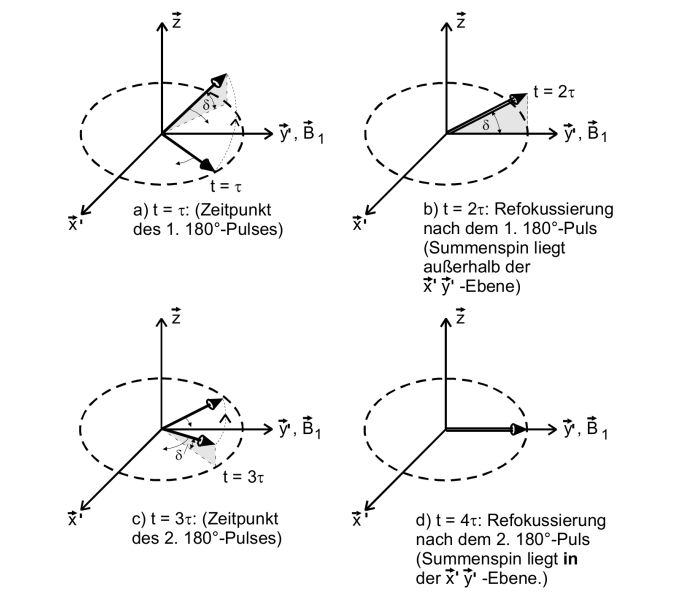
\includegraphics[width=0.8\textwidth]{pics/Meiboom.png}
  \caption{Darstellung des Verhalten der Spins bei der Meiboom-Methode \cite{Anleitung}.}
  \label{fig:Meiboom}
\end{figure}
Diese Methode liefert für alle geradzahlige Echos das richtige $T_2$. Außerdem findet
die Refokussierung in der x-y-Ebene statt, weshalb alle Echos das selbe
Vorzeichen haben. Dies ist bei der Carr-Purcell-Methode nicht der Fall.
\subsection{Spinrelaxation einer flüssigen Probe}
In einer flüssigen Probe muss beachtet werden, dass die sich die Spins auf
Grund der Brownschen Molekularbewegung bewegen und deswegen das statischen Magnetfeld
nicht zeitunabhängig wahrnehmen. Zur Beschreibung muss die Diffusionsstromdichte
\begin{equation}
  \vec{j} = - D\:\nabla\!\left(\frac{N}{V}\right)
\end{equation}
mit der Diffusionskonstante $D$ , der Teilchenzahl $N$ und dem Volumen $V$ definiert werden.
In Verbindung mit den Blochschen Gleichungen ergibt sich für die Änderung der
Magnetisierung
\begin{equation}
  \frac{\partial M}{\partial t} =
  \underbrace{\gamma \left(\vec{M} \times \vec{B}\right)}_{\text{Präzession}}
  \underbrace{- \frac{M_\text{x} \vec{x} + M_\text{y} \vec{y}}{T_2}
  - \frac{\left(M_\text{z} - M_0\right) \vec{z}}{T_1}}_{\text{Relaxation}}
  \underbrace{+ \left(\vec{x} + \vec{y} + \vec{z}\right) D\:\Delta M}_{\text{Diffusion}} .
\end{equation}
Zu dem Magnetfeld wird der Feldgradient $G$  des von außen angelegten Feldes hinzugezogen :
\begin{equation}
  B_\text{z} = B_0 + G z .
\end{equation}
Innerhalb der Probe ist der Gradient $G$ konstant.
So lässt sich der Ausdruck
\begin{equation*}
  M_\text{y}\!\left(t\right) = M_0
  \exp\!\left(- \frac{t}{T_2}\right)
  \exp\!\left(- \frac{t}{T_\text{D}}\right)
\end{equation*}
mit
\begin{equation*}
  T_\text{D} = \frac{3}{D \gamma^2 G^2 \tau^2}
\end{equation*}
für die $y$-Komponente der Magnetisierung gewinnen.
Hierbei ist $\tau$ die Zeitkonstante, wie bei der Carr-Purcell- oder der Meiboom-Gill-Methode, zwischen
dem 90°- und dem 180°-Puls.
Es ergibt sich ein zweiter exponentieller Faktor aufgrund der Diffusion der
zum Zerfall der Magnetisierung beiträgt.
Die Methoden für Festkörper können weiterhin
angewandt werden, wenn $T_\text{D}$ groß gegen $T_2$ ist.
Für die Zeitabhängigkeit der Magnetisierung lässt sich
\begin{equation}
  M_\text{y}\!\left(t\right) = M_0
  \exp\!\left(-\frac{t}{T_2}\right)
  \exp\!\left(-\frac{1}{12} D \gamma^2 G^2 t^3\right)
  \label{eq:DiffusionsBestimmung}
\end{equation}
mit $t = 2\tau$, definieren,
woraus sich bei Variation von $t$ die Diffusionskonstante ermitteln lässt.
